% !TEX root = handbook-physics.tex
% !TEX TS-program = pdflatex
% !TEX encoding = UTF-8 Unicode






\chapter{Magnetic Field Of Direct Current}
\label{ch-23}

\section{Magnetic Field. Ampere's Law}
\label{sec-23.1}

\subsection{}\label{23.1.1} 

A \redem{magnetic field} is one of the forms of an electromagnetic field \ssect{15.1.2}. A magnetic field is set up by moving charged particles, as well as moving bodies carrying electric charges. Magnetic fields act only on moving electric charges and moving charged bodies.

Variable electric fields (displacement currents) \ssect{27.3.1} are
also sources of magnetic fields.

\subsection{}\label{23.1.2} The main force characteristic of a magnetic field is
\redem{vector of magnetic induction} $\vb{B}$ (also called \redem{magnetic flux density}, \redem{magnetic displacement}, or, simply, \redem{magnetic vector}). Vector B is determined by one of three methods:
\begin{enumerate}[label= (\alph*)]
\item from Ampere’s law \ssect{23.1.4};
\item from the effect of the magnetic field on a current-carrying loop \ssect{23.4.2};
\item from the expression for the Lorentz force \ssect{24.1.3}.
\end{enumerate}

\subsection{}\label{23.1.3} Magnetic fields are represented graphically by lines of magnetic induction. \redem{Lines of magnetic induction (lines of magnetic force)} are curves whose tangent at each point coincides with vector $\vb{B}$ at this point of the field. The directions of the magnetic vector and the lines of magnetic induction are determined by the \redem{corkscrew (Maxwell) rule} (also called the \redem{right-hand screw rule}): if a corkscrew with right-hand thread is screwed in the direction of the current density vector in the conductor \ssect{20.2.3}, the direction that the corkscrew handle turns indicates the direction of the lines of magnetic induction and the magnetic vector.

Lines of magnetic induction are not interrupted at any point of the magnetic field, i.e. they neither begin nor end. These lines are either closed curves or they extend from infinity to infinity or they are wound infinitely on some surface, covering it densely all over, but never returning again to any point of the surface. A similar situation is observed, for example, in a field set up by a system of a circular current and an infinite rectilinear current passing through the centre of the circular current and perpendicular to its plane. 

A magnetic field is said to be \redem{uniform}, or \redem{homogeneous}, if vector $\vb{B}$ is constant at any point in the field. Otherwise, it is said to be \redem{nonuniform (nonhomogeneous}).

\subsection{}\label{23.1.4} The force exerted by a magnetic field on a current-carrying conductor placed in the field is called \redem{Ampere's force}. 

\redem{Ampere's law} states that an element of force $\dd \vb{F}$ exerted on a small element of length $\dd l$ of a conductor, carrying a current and located in a magnetic field, is proportional to the vector product of the element $\dd \vb{l}$ of conductor length by the magnetic induction $\vb{B}$:
\begin{align*}%
\dd F & = I \, [\dd \vb{l} \cross \vb{B}] && \text{(in SI units),}\\
\dd F & = \frac{I}{c} \, [\dd \vb{l} \cross \vb{B}]&& \text{(in Gaussian units, see Appendix~I),}
\end{align*}
Here $\dd \vb{l}$ is a vector with the magnitude $\dd l$ and has the same direction as the density vector $\vb{j}$ of the current in the conductor \ssect{20.2.3}.

Ampere’s force $\vb{F}$, acting in a magnetic field on a current-carrying conductor of finite length, is
\begin{equation*}%
\vb{F} = \int I \,  [\dd \vb{l} \cross \vb{B}],
\end{equation*}
in which integration is carried out over the whole length of the conductor. In the case of a uniform magnetic field \ssect{23.1.3}.
\begin{align*}%
\dd F & = I \, Bl \sin \alpha && \text{(in SI units),}\\
\dd F & = \frac{I}{c} \, Bl \sin \alpha && \text{(in Gaussian units),}
\end{align*}
where $\alpha$ is the angle between the density vector of the current in the conductor and vector $\vb{B}$. The relative positions of vectors $\dd \vb{F}$, $\vb{B}$ and $\dd \vb{l}$ are shown in \figr{fig-23-01}. If $\dd \vb{l}$ is perpendicular to $\vb{B}$, the direction of force $\dd \vb{F}$ is found by the \redem{left-hand rule}: if the left hand, opened flat with the fingers parallel to one another and the thumb perpendicular to the fingers, is held so that the magnetic induction vector enters the palm and the fingers indicate the direction of the electric current, the thumb indicates the direction of the force exerted by the magnetic field on the current-carrying conductor. 

It is evident from \figr{fig-23-01} that vector $\dd \vb{F}$ is perpendicular to the plane passing through vectors $\dd \vb{l}$ and $\vb{B}$, and that its direction is such that from the head of vector $\dd \vb{F}$ the direction of shortest rotation from vector d to vector $\vb{B}$ is counter-clockwise. In other words, vector $\dd \vb{F}$ coincides in direction with the vector product $[\dd \vb{l} \cross \vb{B}]$.

\begin{marginfigure}[-2cm]
\centering
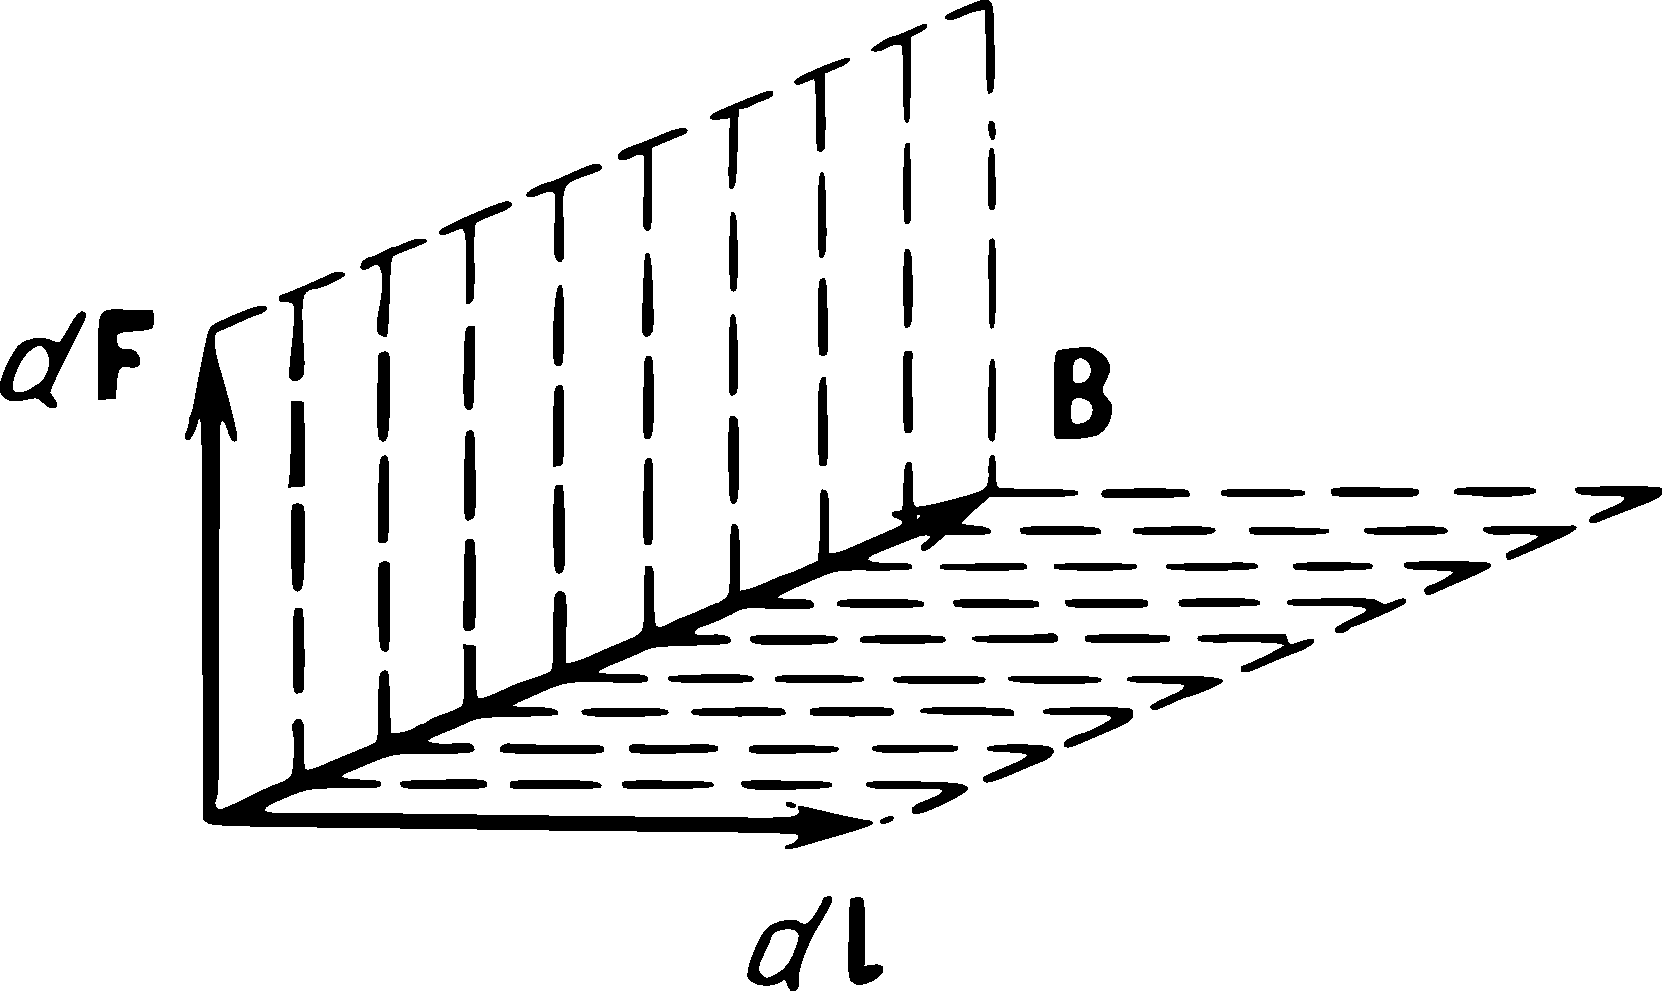
\includegraphics[width=0.9\textwidth]{figs/ch-23/fig-23-01.pdf}
\sidecaption{Directions of vectors $\dd \vb{F}$, $\dd \vb{l}$ and $\vb{B}$.\label{fig-23-01}}
\end{marginfigure}

\subsection{}\label{23.1.5} It follows that the magnetic induction vector in SI units is numerically equal to the limit of the following ratio: the force exerted by a magnetic field on an element of a current-carrying conductor to the product of the current by the length of an element of the conductor, the limit being taken as the length of the element approaches zero and is positioned in the field so that the limit reaches its maximum value. Thus
\begin{align*}%
B & = \frac{1}{I} \, \left( \dv{F}{l}\right)_{\text{max}} && \text{(in SI units),}\\
B & = \frac{c}{I} \, \left( \dv{F}{l}\right)_{\text{max}} && \text{(in Gaussian units),}
\end{align*}
where $c$ is the electrodynamic constant (Appendix~I).

\subsection{}\label{23.1.6} In contrast to electrostatic forces \ssect{14.2.2}, Ampere’s force is not a central one \ssect{3.3.4}. Ampere’s force is perpendicular to the lines of magnetic induction and to the current-carrying conductors.

\section{The Biot-Savart-Laplace Law}
\label{sec-23.2}
 
\subsection{}\label{23.2.1} The Biot-Savart-Laplace law determines the magnetic induction at any point in a magnetic field set up by a direct electric current flowing along a conductor of any shape. The vector dB of magnetic induction at any point C of a magnetic field, set up by an element of a conductor carrying the current I and of the length dl is determined by the formula
dB= kiT [dr],
where d is the vector of an element of length of the conductor \ssect{23.1.4}, r is the radius vector from the element dl of the con­ ductor to point C (Fig. 23.2), r
is the magnitude of the radius
vector r, k is a factor depending only upon the chosen system of units, and iT is a dimension­ less quantity that characterizes the magnetic properties of the medium and called the relative magnetic permeability (or simply relative permeability) of the me­ dium. The relative permeability does not depend upon the choice of units and equals unity for vacu­ um. For all substances, except fer­ romagnetic ones, p,r differs only slightly from unity \ssect{26.5.1}. See
Fig. 23.2
Sect. 26.4.5 for a general defini­
tion of fxr.

\subsection{}\label{23.2.2} In SI units k = (x0/4jt, where p,0 = 4jt x 10~7 henry/m is the permeability of free space, or the magnetic constant (Appen­ dix II). In Gaussian units, k = 1/c, where c = 3 X 1010 cm/s is the electrodynamic constant (Appendix I).
The Biot-Savart-Laplace law is of the form
dB=Ms--£-(rfrr]. 4n H1-1
This form of the Biot-Savart-Laplace law and of all the electro­ magnetic field equations is said to be rationalized.
The product p,0pr is sometimes called the absolute magnetic permeability (or simply permeability) of the medium.
In Gaussian units dB = — — [dl r]. The magnitude of vector
dB is equal to
PoPr / dl sin a CT .. x dB=  -----t*--- SI UIlltS)’
dB—— ? d  a (in Gaussian units), C T*
where a is the angle between vectors dl and r.

\subsection{}\label{23.2.3} The magnetic field strength H is the vector characteristic of a magnetic field that, for a homogeneous isotropic medium, is related to B as follows:
u
H=—— (inSIunits),
H = — (in Gaussian units). Hr
The universal relation between vectors B and H for a magnetic field in an arbitrary medium and the more general definition of the magnetic field strength vector H are discussed in Sect. \ssect{26.4.4}.
The strength of a magnetic field set up by a direct current in a homogeneous isotropic medium is independent of the magnetic properties of the medium. Thus
PoPr g
7tt 1 rjii j»Idlsina
.. (ln SI unlts)>
Gaussian units),
where a is the angle between vectors dl and r.

\subsection{}\label{23.2.4} It follows from a comparison of the characteristics of electric (E and D) and magnetic (B and 11) fields that the electric field strength vector E is analogous to the magnetic vector B. Both vectors specify the force effects of the fields and depend upon the properties of the medium in which the field is set up.
The analogue of vector D of electric displacement \ssect{15.3.1} is fhe magnetic field strength vector II,
[dl r]’ dH= rfH=— [dl r], dll=
4nr2
sina cr3 cr2

\subsection{}\label{25.2.5} An electric charge g, travelling in an unbounded homo­ geneous and isotropic medium at the constant velocity v, sets up a magnetic field whose magnetic induction Bg can be cal­culated by the formula"
where (3is the angle between vectors v and r, and r is the radius vector from the travelling charge to the point A being considered in the field. Vectors Bq and Hg are perpendicular to the plane passing through vectors v and r.
When q > 0, the shortest rotation from vector v to vector r is seen from the head of vector Bg (and Hg) to be counter­
Fig. 23.3

clockwise (Fig. 23.3a). When q < 0, then B  (and Hg) have the opposite direction (Fig. 23.3b). The magnetic field of a moving charge is variable, because the radius vector r varies in magnitude and direction as charge q travels even if v = const. The magnetic field of a moving charge, depending upon angle (3 between vectors v and r, is not spherically symmetrical, as in the case of the electrostatic field of a point charge \ssect{14.2.3}. The magnetic field being considered has mirror symmetry with respect to the direction of v. The field strength is maximum at points in a plane passed through the charge perpendicularly to vector v (under the condition that u<c c). At all points on a straight line coinciding with vector v there is no magnetic field induction,

\section{Simplest Cases of Magnetic Fields Set Up by Direct Currents}
\label{sec-23.3}

\subsection{}\label{23.3.1} Making use of the Biot-Savart-Laplace law we can deter­ mine the characteristics (B and H) of a magnetic field set up by
M
an electric current flowing in a conductor of finite dimensions and arbitrary shape. According to the principle of superposition of fields \ssect{15.2.2} the magnetic induction B at an arbitrary point of a magnetic field of a conductor carrying the current I is equal to
B
B -5dB
where dB is the magnetic induction
of the field set up by an element
of the conductor with the length dl. Integration is carried out over the
whole length L of the conductor.

\subsection{}\label{23.3.2} A straight conductor MN car­ rying the current I sets up a mag-
//
l Fig. 23.4
netic field with induction B and strength H at an arbitrary point A equal to*
B= —(cosCD-.—costp2), H=  --(inSIunits), r0   i0[ir
IIB
B——ur— (coscpj—coscp2), H=— (inGaussianunits),
c r0 Mr
where rQis the distance from point A to the conductor, q)x and cp2are the angles formed by the radius vectors from point A to the beginning and end of the conductor (Fig. 23.4), ir is the
* It is assumed in all the examples of Sect. \ssect{23.3} that the medium is homogeneous, isotropic and completely fills all the space in which the magnetic field exists.
relative magnetic permeability of the medium, and p0is the magnetic constant in SI units (Appendix II).
For an infinitely long conductor (q)x = 0 and (p2 = xt)
B= HoHr 2/ B (in SI units), 4n HoHr
Z?= — Ur — , H = - ~ (in Gaussian units). c r0 Hr

\subsection{}\label{23.3.3} For the magnetic field at the centre of a rectangular turn (loop) carrying the current I
Wr 81Ya2+b2
H ——-— (in SI units), HoHr
H = — (in Gaussian units), Hr
4tt
ab
8
ab
where a and b are the sides of the rectangle.

\subsection{}\label{23.3.4} The magnetic moment pm of a closed loop of arbitrary shape, carrying the current /, is equal to
pm = / j n dS, (in SI units), s
pm= - -/ J ndS (in Gaussian units), s
where n is a unit vector of the outward normal to element dS of the surface S , bounded by the current-carrying loop. In the case of a flat loop, surface S is plane and all the normals have the same direction. Hence
pm= ISn, pm= IS (in SI units),
11
pm= —ISn, pm= —IS (in Gaussian units).
99
Vector pm is directed so that from its head the current in the circuit is seen to be flowing counterclockwise (Fig. 23.5).


\subsection{}\label{23.3.5} The magnetic field set up by a circular turn, or loop, carrying the current /, at an arbitrary point A on the axis of the turn (loop) (Fig. 23.6), is specified by
B=.PqHt-   , H= B (inSIunits),
4ri (R2+ h2)3/2
2d b
|ix0|Ltr v '
B= (Xr(fl2+T2)3/2’ H="fl7 (in Gaussian units)-
Here pm is the magnetic moment of a current-carrying turn, or loop, \ssect{23.3.4}.

The magnitudes of vectors B and H equal
i0ir IR 2   x0xrIS
2 (/?2+fr2)3/2 2JX(i?2+ 2)3/2’
H = ----- (in SI units), PoPr
1 2nIR2 1 2IS c r(i?2+*2)3/2—c  (fl2+/i2)3/2
If = — (in Gaussian units), Pr
whore h is the distance from point A to the centre of the turn (loop), R is the radius and S is the area of the turn.

\subsection{}\label{23.3.6} The magnetic field at the centre of a circular turn, or loop, has the characteristics \ssect{23.3.5}:
fWr 2pm 4n i?3
g
H= ---- (in SI units),
M-oMt
H= f*r 2pm
Ihe magnitudes of vectors B and II equal
= JR ' H = 2  (in SI units)> 2R
 2it I
11= ~ ' (in Gaussian units).
H = — (in Gaussian units). i?3’ Mr
The direction of the magnetic field is along the axis of the loop and perpendicular to its plane (Fig. 23.6).
Fig. 23.7

\subsection{}\label{23.3.7} A toroid is an annular coil wound on a core having the shape of a torus (Fig. 23.7). The magnetic field of a toroid is completely confined within its volume,

The characteristics of this magnetic field are calculated by the formulas
D NI TT NI OT .4x B=  t2nr' H=z~2nr(lnSIunlts)’
„ 1 2NI TT 1 2NI (in Gaussian units). cic
The magnetic induction B and the strength H of the magnetic field on the circular centre line of the toroid are equal to
NI
H= nl (in SI units).a
Here N is the number of turns of the toroid, I is the current in the turns, r is the radius of a circle in the toroid, Rc= = (/?! -f   2)/2, and i?2 are the external and internal radii of the torus, and n is the number of turns per unit length of the toroid’s centre line.

\subsection{}\label{23.3.8} A solenoid is a cylindrical coil consisting of a large number of turns of wire in the form of a helix. If the turns are wound tight up against or sufficiently close to one another, the solenoid is dealt with as a system of circular closed current-carrying loops connected in series and having the same radius and a common axis.

The magnetic moment pm \ssect{23.3.4} of the solenoid is equal to the vector sum of the magnetic moments of all N of its turns. Thus
Pm= NISn,
where I is the current in the solenoid’s turns, S is the area of a turn, and n is a unit vector of the normal to the plane of a turn. Vector pm is along the axis of the solenoid and coincides in direction with the magnetic field as determined by the cork­ screw rule \ssect{23.1.3}.

The magnetic induction B and strength H of the solenoid’s magnetic field at an arbitrary point A, lying on its axis, are

numerically equal to
//— -nl(cosa2—cosaj), H= B-(inSIunits),
1B
/> —2jqir/i/r(cosa2—cosocj), H= — (in Gaussian units),
C Hr
where n — N/L is the number of turns per unit length of the solenoid, a2and axare angles at which the ends of the solenoid nro seen from point A (a2< ax),
cosa1= -------------, cosa2= — L—U — , VR2+ ll /«*+ (/.—*!)*
// is the length of the solenoid (Fig. 23.8), and R is the radius of the cylindrical coil.
Fig. 23.8

\subsection{}\label{23.3.9} Under the condition that L > /?, the magnetic field inside the solenoid at points on its axis sufficiently distant from its ends is characterized by the values
B=i0rnI, II=nI(inSIunits),
11
B= —- H= —£nnI (in Gaussian units).
 302

The magnetic induction B and strength H of the magnetic field of a solenoid of sufficient length, at points of its axis coinciding with its ends, are equal to
B= —-nT, H=±nl(inSIunits),
11
B=—2n,TnI, Ii=—2nnl (ingredients).

\section[Interaction of Conductors]{Interaction of Conductors. Effect of a Magnetic Field on Current-Carrying Conductors}\label{sec-23.4}

\subsection{}\label{23.4.1} Ampere’s force \ssect{23.1.4}, which acts on an element dl of length of a straight conductor carrying the current Ilt and is exerted by a long straight conductor carrying the current /2, located parallel to the first conductor at a distance of a, is numerically equal to
d/?= -M!2L l±dl (in SI units), 4jia v7
1 21I
dF= — ij:— (in Gaussian units),
where |i0 is the magnetic constant in SI units \ssect{23.2.2} and c is the electrodynamic constant (Appendix I). The force dF is a force of magnetic interaction \ssect{24.1.4}.

It is assumed that the lengths of the conductors are many times greater than the distance a between them, and that element dl is located far from the ends of the first conductor. It is moreover assumed that the conductors are in a homogeneous isotropic medium having the relative magnetic permeability p,r.
The force F exerted on a current-carrying conductor of length I is equal to
21ih t (in SI unitS) 4nav 7
1 21I
F=- -ir —  -2-1 (in Gaussian units).
Conductors carrying currents /i and I 2 that flow in the same direction attract each other. If the currents flow in opposite directions, the conductors repulse each other (see also Sect. \ssect{24.1.4}).

\subsection{}\label{23.4.2} A closed flat current-carrying loop, of arbitrary geometric shape, placed in a uniform magnetic held \ssect{23.1.3}, is subjecf to a moment of force (t orque) M equal to
M = [PmB],
where pm is the magnetic moment vector of a current-carrying loop \ssect{23.3.4}, and B is the vector of magnetic induction \ssect{23.1.2} of the held. Torque M is perpendicular to the plane passing through vectors pm and B in such a manner that the shortest rotation from pm to B is seen from the head of vector M to be counterclockwise. The torque tends to turn the loop to a position of stable equilibrium, in which vectors pm and B are parallel to each other.
The preceding formula provides for a definition of the magnetic induction B \ssect{23.1.2}: the magnitude of the magnetic induction vector at a given point of a uniform magnetic field is equal to the maximum value of the torque Afmax acting in the vicinity of the point on a small flat closed current-carrying loop, having a magnetic moment pm of unit magnitude:
B—  max   l max (in SI units), Pm .IS
B= - max   Mmax (in Gaussian units).
Pm —IS c

\subsection{}\label{23.4.3} When a closed current-carrying loop is placed into a nonuniform magnetic field \ssect{23.1.3} in which the magnetic induction B of the field varies over distances comparable to the linear dimensions of the loop, the loop is subject to the force F equal to
where pmx, pmv and pmz are the projections of vector pm on the axes of Cartesian coordinates. In particular, when vector B
is along the OX axis and depends only on coordinate x [i.e. Bx—B(a;),By—Bz—0and B= then
  dB. Y~ Pmxi t e u
By the action of force F an unfastened current-carrying loop is attracted into a region with a stronger magnetic field.

\section{Total Current Law. Magnetic Circuits}
label{sec-23.5}

\subsection{}\label{23.5.1} The circulation of the magnetic induction vector B along a closed circuit L is an integral of the form:
< )Bd= ( )Bdcosa,
LL
where L is the closed loop of arbitrary shape, a is the angle between vectors B and dl, and d is the vector of an element of length of the loop in the direction it is circuited.
\subsection{}\label{23.5.2} The total current law for a magnetic field in vacuum states: the circulation of the magnetic induction vector of a magnetic field along a closed loop in vacuum is proportional to the alge­ braic sum of the currents bounded by the loop. Thus
n
 )Bdl=|x02 Ih(inSIunits),
L
L
= y
fc=l n
  Ik (in Gaussian units), h= 1
where (i0is the magnetic constant in SI units \ssect{23.2.2}, c is the electrodynamic constant \ssect{23.2.2} and n is the number of current-carrying conductors bounded by loop L of arbitrary shape. This law is valid for current-carrying conductors of any shape or size.
In calculating the algebraic sum of the currents, a current is considered positive if from the head of the current density
vector \ssect{20.2.3} the circuiting of loop L is seen to be counter­ clockwise. Otherwise, the current is considered to be negative. For a generalization of the total current law to cover magnetic fields in an arbitrary media, see Sect. \ssect{26.4.2}.

\subsection{}\label{23.5.3} In contrast to an electrostatic conservative field, in which the circulation of the strength E along any closed path equals zero (\ssect{16.1.4}), a magnetic field has a curl (it is called a rotational, vortical or circuital field). In such a field the cir­culation of the magnetic induction vector B of the field along a closed path is not equal to zero. If no currents are bound by loop L, the circulation of vector B along this loop equals zero. But this does not alter the rotational nature of the magnetic field.

\subsection{}\label{23.5.4} The total current law can be written for either vacuum or for an arbitrary medium in the form of the circulation of field strength vector H (\ssect{23.2.3}) along an arbitrary closed loop L that bounds the currents:
n
L h=1 n
L k=l
If no currents are bounded by loop L, the circulation of vector H along this loop equals zero.

\subsection{}\label{23.5.5} The flux of the magnetic induction vector B (magnetic flux) through a surface element of area dS is the scalar physical quantity equal to
dOm = B dS = Bn dS = B dS cos y,
where dS = n dS, n is the unit vector of the normal to the surface of area dS, Bn is the projection of vector B on the direc­ tion of the normal (Fig. 23.9), and y is the angle between vec­ tors B and n. The magnetic flux (Rm through an arbitrary sur­ face S is

In calculating this integral, the vectors n of the normals to the elements of surface dS should be all in the same direction with respect to surface S. Thus, if S is a
closed surface, vectors n should be direct­ ed either all outward or all inward. When the field is uniform and S is a plane surface perpendicular to vector B,then Bn=B=const and Om= —BS.

\subsection{}\label{23.5.6} The 0sirogradsky-Gauss
for a magnetic field states that the magnetic flux through an arbitrary closed surface equals zero.
Thus
<£BdS= BndS=0.
This theorem is a mathematical expression of the fact that in nature there are no magnetic charges at which lines of magnetic induction begin or end (\ssect{23.1.3}).
The differential form of the Ostrogradsky-Gauss theorem for a magnetic field is one of Maxwell’s equations for an electro­ magnetic field \ssect{27.4.2}.

\subsection{}\label{23.5.7} A magnetic circuit is a set of bodies or regions of space to which a magnetic field is confined. For example, the internal region of a toroid \ssect{23.3.7} and that of an infinitely long solenoid \ssect{23.3.9} are magnetic circuits. To strengthen their magnetic fields, magnetic circuits are made of materials having a high relative magnetic permeability p,r \ssect{23.2.1}, such as iron. The design of magnetic circuits, which are the essential components of electrical machinery and such electric devices as transformers and electromagnets, is based on the laws of magnetic circuits. 

\subsection{}\label{23.5.8} Ohm's law for a closed magnetic circuit (the Hopkinson
formula) is
where Om is the magnetic flux, which is constant along each portion of the magnetic circuit, Fm = IN is the magnetomotive force (mmf)y or magnetizing force (in SI units), N is the number of turns carrying the electric current I for magnetizing the
circuit, and Rm is the total magnetic resistance reluctance) of ike circuit. The magnetic resistance of a magnetic circuit of length li is
hf dl
Nml== J l   s - (ln SI umts)’
0
where p,r is the relative magnetic permeability of the given circuit, |x0 is the magnetic constant in SI units \ssect{23.2.2}, and S is the cross-sectional area of the circuit. When S = const,
i = li/iTS (in SI units).

\subsection{}\label{23.5.9} The total magnetic resistance Rm of the parts of a mag­ netic circuit connected in series is
n
Rm—2 ii» i=1
where i?mi is the magnetic resistance of the ith part of the mag­ netic circuit, and n is the number of parts that make up the circuit.
If n magnetic resistances are connected in parallel, the total magnetic resistance Rm of the circuit is
y—-   Rmi
2=1

\subsection{}\label{23.5.10} A branch point of a magnetic circuit is a region of space or bodies where there are more than two possible directions of the lines of magnetic induction \ssect{23.1.3}.
Kirchhoff's first law for branched magnetic circuits states that the algebraic sum of the magnetic fluxes in the branches that join in a branch point is equal to zero. Thus
J a>ml = 0, 2= 1
where n is the number of branches joined at the branch point (cf. Sect. \ssect{23.3.1}).
20*
A magnetic flux is considered positive if the lines of induction enter the branch point, and negative if the lines emerge from it. 

\subsection{}\label{23.5.11} Kirchhoff's second law for magnetic circuits states that in any closed loop (mesh of a network), arbitrarily chosen in a branched magnetic circuit (network), the algebraic sum of the products of the magnetic fluxes by the magnetic resistances of the corresponding portions of the circuit \ssect{23.5.8} equals the algebraic sum of the magnetomotive forces in this loop \ssect{23.5.8}:
kk
2=1 2=1
where k is the number of portions that make up the closed loop (cf. \ssect{21.3.2}). The fluxes and mmf’s F i are considered po­ sitive if the directions of the corresponding lines of magnetic induction \ssect{23.1.3} coincide with the arbitrarily chosen direc­ tion for circuiting the loop.

\section[Work Done in a Magnetic Field]{Work Done in Moving a Current-Carrying Conductor in a Magnetic Field}
\label{sec-23.6}

\subsection{}\label{23.6.1} An unfixed current-carrying conductor is moved by Ampere’s force \ssect{23.1.4} when it is placed in a magnetic field. The element of work done by the Ampere force in moving an element, of length dZ, of a conductor carrying the current I is
6 *=/ *, (inSIunits),
1
6PF* = —-/ dcDj  (in Gaussian units),
where dO  is the element of magnetic flux \ssect{23.5.5} through the element of surface dS generated by the element of the conductor, of length dZ, in its small displacement, and c is the electrody­ namic constant \ssect{23.2.2}.

\subsection{}\label{23.6.2} In a small displacement of a current-carrying conductor of finite length, the work 6W done by the Ampere forces is the sum of the elements of work for all the elements of length of the
conductor. It is equal to the integral of 6W* calculated along llie whole length I of the conductor. Thus
(W= j I(10 =1j d<D*l= Id<Dm (in SI units), ll
1
hW= — I dd)m (in Gaussian units),
c
where d<3>m is the magnetic flux through the surface generated by the conductor of length I in a small displacement.

\subsection{}\label{23.6.3} If a conductor of finite length I carries a constan tcurrent I and is moved a finite distance, the required work of the Ampere forces for this motion is
W= /(Dm,
where Om is the magnetic flux through the surface generated by the conductor in its motion.

\subsection{}\label{23.6.4} The work done by Ampere forces in the displacement of a closed flat loop carrying the constant current / in a magnetic field from initial position 1 to final position 2 is equal to
If12 = I ((f)m2 — (l)mi)>
where Omi and  m2 are magnetic fluxes “linked to the loop” in positions 1 and 2, i.e. the magnetic fluxes through a surface bounded by the loop. In calculating these magnetic fluxes, the direction of normal n \ssect{23.5.5} is coordinated with the direction of the current in the loop by the corkscrew rule: from the head of the vector of the normal, the current is seen flowing counter­ clockwise in the loop.

\subsection{}\label{23.6.5} The formulas given above are valid for a current-carrying coil of N turns moving in a magnetic field by Ampere forces, or, in general, for a loop of arbitrary shape. For example, the work done in a small displacement of a coil carrying the current I is equal to
m =i 2d®mi=id(v1a>mi)=idv, i=l i—i
NN
where W = y] <S>mi is the total magnetic flux through all N
i=l
turns of the coil; it is called the flux linkage of the circuit. 

\subsection{}\label{23.6.6} The work required to move a conductor or closed loop carrying a constant current in a magnetic field is done at the expense of the energy consumed in the current source \ssect{21.1.3}.